% !TEX root = main.tex

\begin{figure}
    \centering
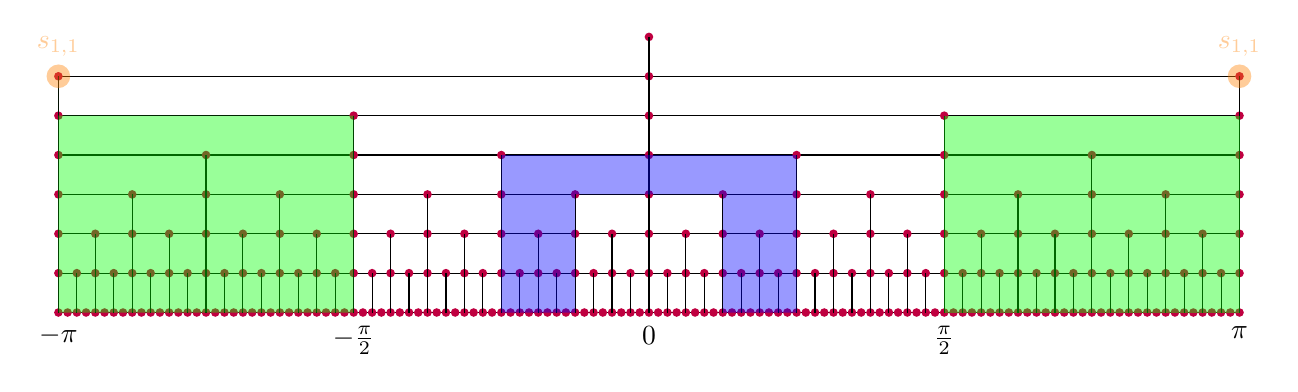
\begin{tikzpicture}[scale=0.5]

  \pgfmathsetmacro{\xlimit}{30}
  \pgfmathsetmacro{\ylimit}{7}

  \foreach \yunscaled in {0,..., \ylimit} 
  {
    \pgfmathsetmacro{\y}{\yunscaled}
    \pgfmathsetmacro{\lognumpoints}{\ylimit-\y}
    \pgfmathsetmacro{\numpoints}{2^\lognumpoints}
    \pgfmathsetmacro{\z}{\xlimit/\numpoints}
    \ifnum\y=\ylimit{
      % Do nothing
    }
    \else{
      \draw (0,\y) -- (\xlimit,\y);
      \foreach \i in {0,...,\numpoints}{
        \pgfmathsetmacro{\x}{\z * \i}
        \draw (\x,\y) node[circle,fill,inner sep=1.1pt, color=purple]{}; % Marked point
      \draw (\x,\y) -- (\x,0); % Vertical line
      }
    }
    \fi
  }
  \draw (\xlimit/2,\ylimit) node[circle,fill,inner sep=1.1pt, color=purple]{}; % Marked point
  \draw (\xlimit/2,\ylimit) -- (\xlimit/2,0); % Vertical line


  % Label horizontal lines
  \draw (0,-0.1) node[below] {$-\pi$};
  \draw (\xlimit/4,-0.1) node[below] {$-\frac \pi 2$};
  \draw (\xlimit/2,-0.1) node[below] {$0$};
  \draw (\xlimit*3/4,-0.1) node[below] {$\frac \pi 2$};
  \draw (\xlimit,-0.1) node[below] {$\pi$};

\fill [green, opacity=0.4] 
  (0,\ylimit-1)
  --(0,\ylimit-2) 
  -- (\xlimit/4,\ylimit-2)
   -- (\xlimit/4,\ylimit-7)
  -- (0,\ylimit-7)
  --cycle;  

\fill [blue, opacity=0.4] 
(\xlimit/4+\xlimit/8, \ylimit-3)
-- (\xlimit/4+\xlimit/8, 0)
-- (\xlimit/4+\xlimit/8+\xlimit/16, 0)
-- (\xlimit/4+\xlimit/8+\xlimit/16, \ylimit-4)
-- (\xlimit/4+\xlimit/4+\xlimit/16, \ylimit-4)
-- (\xlimit/4+\xlimit/4+\xlimit/16, 0)
-- (\xlimit/4+\xlimit/4+\xlimit/8, 0)
-- (\xlimit/4+\xlimit/4+\xlimit/8, \ylimit-3)
--cycle; 

\fill[orange, opacity=0.4] (\xlimit, 6) circle (0.3) node[label={[]:$s_{1,1}$}]{};

\fill[orange, opacity=0.4]
(0, 6) circle (0.3) node[label={[]:$s_{1,1}$}]{};


\fill [green, opacity=0.4] 
        (\xlimit-0,\ylimit-2)
    -- (\xlimit-\xlimit/4,\ylimit-2)
    --(\xlimit-\xlimit/4, \ylimit-7)
    --(\xlimit, \ylimit-7)
    -- cycle;



  % \tikzmath{
  %   \curx = 0;
  %   for \step in {1,...,2}{
  %     {\draw [magenta,-, double=magenta, double distance=4\pgflinewidth, opacity=0.4] (\curx, \ylimit-\step) -- (\curx, \ylimit-\step-1);};
  % };}
  
\end{tikzpicture}
\captionof{figure}{
Using the dyadic representation from \cref{fig:dyadic_grid},
 the domain $\mathcal U_{-1}$ is highlighted in green, and the domain $\mathcal K_{3,4}$ is highlighted in purple.
 The station $s_{1,1}$ is highlighted in orange; recall that points with external angle $\pm \pi$ appear twice in this representation. 
 %Also notice that every itinerary passing through the station $s_{1,1}$ must continue vertically from it.
 }  \label{fig:dyadic_grid_regions}
\end{figure} 
